\chapter{Implementation}
Nun da die Grundlagen gelegt sind können wir anfangen zu untersuchen wie ein LSTM Netz mit Events umgeht. Wir betrachten dazu das Bouncing Ball Szenario, da es klare Events hat und sich dadurch auch gut segmentieren lässt. Zur Implementation wurde JANNLab (Otte et al. 2013), ein Java Framework für Neuronale Netze verwendet \cite{bib:jannlab}. Dieses Kapitel soll die im Zuge dieser Arbeit verwendeten Techniken erklären und aufzeigen wie die im nächsten Kapitel beschriebenen Ergebnisse erreicht wurden, sowie welche Probleme sich dabei in den Weg gestellt haben.

\section{Das Bouncing Ball Szenario}
Das Bouncing Ball Szenario beschreibt einen Ball, der gleichförmig durch die Ebene gleitet bis er an entsprechenden Begrenzungen abprallt. Wir haben die 1- und die 2-dimensionale Version verwendet.

Im 1-D Fall haben wir einen Ball ohne Ausdehnung (also eigentlich ein Punkt aber diese Unterscheidung ist für unsere Zwecke irrelevant) mit einer Position $ x_{b} $ und einer konstanten Geschwindigkeit $  v$. Dieser springt zwischen den Grenzen $ x_{1}=-1 $ und $ x_{2}=1 $ hin und her, also immer wenn die Position des Balls eine der Grenzen annimmt, wird die Geschwindigkeit invertiert $ v := -v $. Also genau so wie man es sich vorstellt.

Der 2D Fall funktioniert analog, der Ball hat eine Position $ (x_{b}/y_{b}) $, eine konstante Geschwindigkeit $ (v_{x}/v_{y}) $, welcher nun zwischen den 4 Grenzen $ x_{1}=-1 $ und $ x_{2}=1 $, $ y_{1}=-1 $ und $ y_{2}=1 $ hin und her springt. Nimmt nun eine Koordinate des Balls eine der Grenzen an wird die entsprechende Koordinate invertiert, also $ (v_{x}/v_{y}) = (-v_{x}/v_{y}) $ beziehungsweise $ (v_{x}/-v_{y}) $. 

Das 1D-Szenario habe ich hauptsächlich verwendet um mich einzuarbeiten und zurechtzufinden, da es unter anderem mit weniger Neuronen erlernt werden kann und so die Aktivierungen der einzelnen Gates auch übersichtlicher sind. Der Grund warum das 1D-Szenario auch für diese Ausarbeitung wichtig ist, ist das unter Hinzunahme der Zeitachse aussagekräftige Diagramme erstellt werden können, anhand derer einige Trainingseffekte und Verläufe veranschaulicht werden können. Entsprechende Analysen konnten vom 2D-Fall auch gemacht werden, wenn man sah wie sich eine Linie oder ein Ball mit Verzögerung entsprechend über den Bildschirm bewegt, die resultierenden Bilder sind jedoch eher unübersichtlich. Das 2D Szenario hingegen ist das für unsere Untersuchungen interessantere, da es mehr Events gibt, die auch in komplexernen Beziehungen zueinander stehen. In Abbildung \ref{img:1dvs2d} sieht man jeweils 2 Beispiele, zu dem genauen Aufbau des dazu benutzten LSTM Netzes kommen wir in der folgenden Sektion.
\begin{figure}
	\centering
	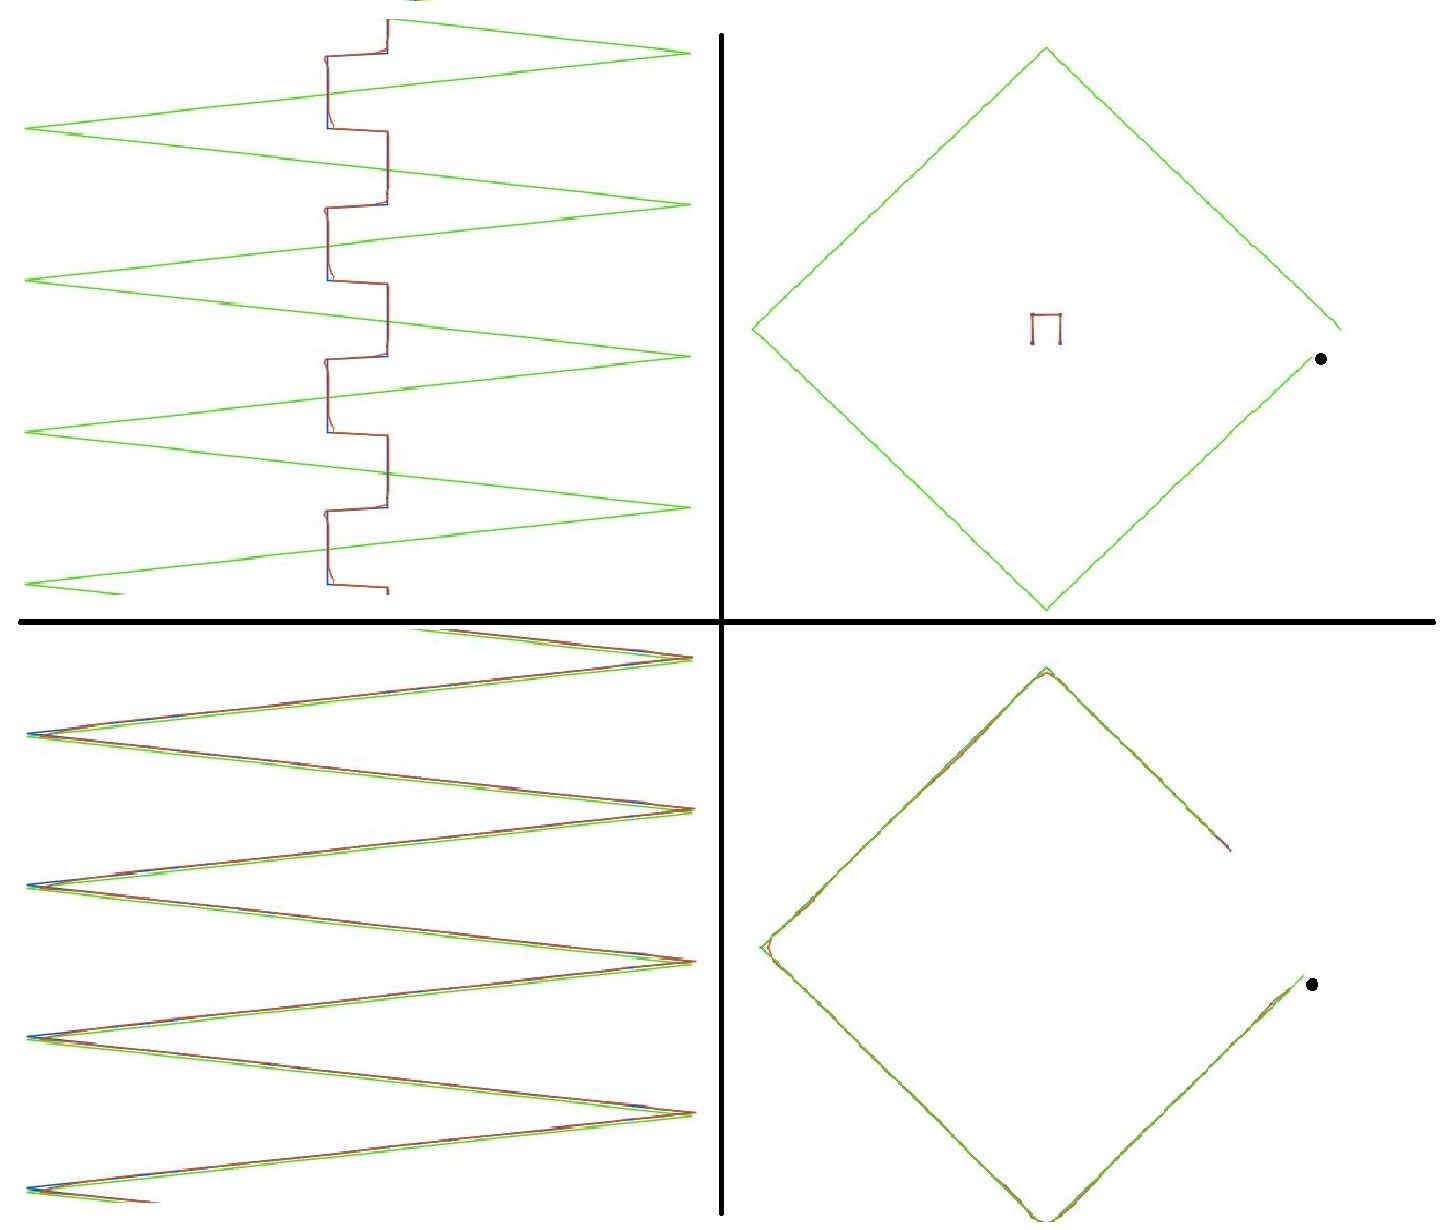
\includegraphics[width=0.9\textwidth, height=370px]{pics/1dvs2d.jpg}	
	\caption{4 Versionen des Bouncing Ball Szenario erlernt durch LSTM Netze. Zu sehen sind der Netzinput (grün), der Netzoutput (rot) und das Trainingsziel (blau). Links sieht man 2 Beispiele des 1D Falls, zur besseren Veranschaulichung sind die Daten nach den Zeitschritten vertikal versetzt. Rechts sieht man 2 Beispiele des 2D Falls, die Abbildung zeigt jeweils den Verlauf des Balls bis kurz vor dem vollenden einer Runde, um Überlagerungen in der Abbildung zu vermeiden. Der Startpunkt ist durch den schwarzen Punkt gekennzeichnet. In den jeweils oberen Fällen wurde als Netzinput die Position des Balles und als Trainingsziel die Geschwindigkeit des Balles für den nächsten Schritt. In den jeweils unteren Fällen wurde als Netzinput die Position des Balles und als Trainingsziel die vorauszuberechnende nächste Position des Balles.}
	\label{img:1dvs2d}
\end{figure}

\section{Unser LSTM, Parameter + Testfälle}
Für unser LSTM-Netz haben sich folgende Parameter als sinnvoll erwiesen:
\begin{description}	\item[Aktivierungsfunktionen:]\hfill \\ 
	Zur Ansteuerung der Gates der LSTM-Zellen im Hiddenlayer werden Neuronen mit \textit{Tangens hyperbolicus} als Aktivierungsfunktion verwendet. Für das Outputlayer wird zur Aktivierung die lineare Funktion verwendet, da die Position des Balles gleichverteilt Werte zwischen -1 und 1 annimmt, soll unser Netzoutput dasselbe tun. Anfangs war für das Outputlayer per Defaultoption die \textit{sigmoid}-Funktion zur Aktivierung eingestellt, deren Bild aber nur von 0 bis 1 reicht. Das hatte natürlich nicht funktioniert und für Verwirrung gesorgt, warum denn nur die Hälfte des Problems erlernt wird.  
	\item[Trainingsoptimierung:]\hfill \\ 
	Als Optimierungsmethode für das Traing wurde die Adaptive Moment Estimation Methode(ADAM), also eine adaptive Momentumsschätzung, verwendet. Diese baut die übliche Lernmethode mit Lernrate und Momentumrate dahingehend aus, dass diese durchgehend angepasst werden, um noch schneller zu genaueren Ergebnissen zu kommen. Hierzu wurden die Standard Parameter verwendet, also $ \beta_{1}=0.9, \beta_{2}=0.99 $ und $ \epsilon = 10^{-8}$. Wobei $ \beta_{1} $ und $ \beta_{2} $ die Abklingraten des Einflusses der vergangenen Momenti auf den jetztigen Zeitschritt sind. Sind sie Nahe 1, klingt der Einfluss langsamer ab. $ \epsilon$ ist ein glättender Term, der Division durch 0 verhindert. \cite{bib:adam} Es wurde für Debugging-Zwecke an diesen Werten herumgespielt, es wurden aber nie sichtlich bessere Ergebnisse erzielt.
	\item[Netzgröße:]\hfill \\ 
	Die passende Netzgröße ist  fallabhängig, in Abbildung \ref{img:1dvs2d} wurden für die 1D Fälle 1-2-1 Netze verwindet (also 1 Inputneuron, 1 Hiddenlayer mit 2 Neuronen und 1 Outputneuron), für die 2D Fälle 2-4-2 Netze. An anderer Stelle werden andere Netzgrößen verwendet, dann wird das an entsprechender Stelle auch nochmal aufgegriffen.
	\item[Außerdem:]\hfill \\
	Alle Layer sind mit Bias-Unit, um mit möglichst wenig Neuronen möglichst viel Funktionalität zu erreichen, damit deren Analyse wiederrum möglichst ausgiebig verläuft. Peepholes \cite{bib:lstm2} wurden getestet, hatten in diesem Beispiel keinen sichtbaren Effekt auf das Training und wurden dann weggelassen.  
\end{description}
Außerdem wurden verschiedene Testfälle mit verschiedenen Intentionen betrachtet, die ich aber an dieser Stelle vorgreifend definieren möchte:
\begin{description}
	\item[Verschiedene Inputs:]\hfill \\
	
	\item[Verschiedene Outputs:]\hfill \\
	
	\item[Zufällige Startposition + Geschwindigkeit:]\hfill \\
	
	\item[Feedback:]\hfill \\
\end{description}


\section{Das Training des Bouncing Verhaltens}

\section{Umfragen zum Thema}
1 von 1 befragten Personen mit einem Abschluss in Bachelor of Science meinten zum Thema: \\
Davon weiß ich nichts. \cite{bib:lstm}


\section{Feedback}



Das Training des Bouncing Verhaltens
Das interessante am Bouncing Ball Szenario ist natürlich nicht die gleichförmige Bewegung, sondern das nicht-lineare Verhalten beim Abprallen. Dieses wollen wir unserem LSTM Netzwerk möglichst genau erlernen und haben dazu einige Techniken angewendet. 

Reaktives vs vorhersehendes Verhalten
1D mit 1b Zelle

RNN Annäherung vs echte nichtlinearität
Random vs nicht Random, nur periodisch gelernt
Feedback für random, erklären warum es nicht funkltioniert hat,
Feedback, Zittern erklären für Input außerhalb des eigenen Raums
Schritte damit es funktioniert, feedback annäherung, hat nicht geholfen
Random diskretisiert um numerisch genau definiertes Rand verhalten zu haben